\documentclass{article}

\usepackage{amsmath}
\usepackage{amssymb}
\usepackage{amsthm}
\usepackage{amssymb}
\usepackage{mathdots}
\usepackage[pdftex]{graphicx}
\usepackage{fancyhdr}
\usepackage[margin=1in]{geometry}
\usepackage{multicol}
\usepackage{bbm}
\usepackage{esint}
\usepackage{listings}
\PassOptionsToPackage{usenames,dvipsnames}{color}  %% Allow color names
\usepackage{pdfpages}
\usepackage{algpseudocode}
\usepackage{tikz}
\usepackage[T1]{fontenc}
\usepackage{inconsolata}
\usepackage{framed}
\usepackage{wasysym}
\usepackage[thinlines]{easytable}
\usepackage{wrapfig}
\usepackage{hyperref}
\usepackage{cancel}
\usepackage{tabu}
\usepackage{tabularx}
\usepackage{mathtools}
\usepackage{mathrsfs}
\usepackage{enumerate}
\usepackage{enumitem}
\usepackage{tabto}

\renewcommand{\P}{\mathbb{P}}
\DeclareMathOperator{\N}{\mathbb{N}}
\DeclareMathOperator{\Z}{\mathbb{Z}}
\DeclareMathOperator{\Q}{\mathbb{Q}}
\DeclareMathOperator{\R}{\mathbb{R}}
\DeclareMathOperator{\C}{\mathbb{C}}
\DeclareMathOperator{\F}{\mathbb{F}}
\DeclareMathOperator{\E}{\mathbb{E}}

% Margins
\topmargin=-0.45in
\evensidemargin=0in
\oddsidemargin=0in
\textwidth=6.5in
\textheight=9.0in
\headsep=0.25in

\title{Problem Set 3}
\author{Laker Newhouse\\Collaborators: Evelyn Fu, Jacob Hansen}
\date{\today}

\begin{document}
\maketitle	

All code and raw results are available at \url{https://github.com/Arongil/6.S098/tree/main/pset3}.
\begin{enumerate}
    \item We formulate the problem of finding the maximum likelihood estimate of $x$ given $y$ as a convex optimization problem as follows. We let $x$ be the problem variable. It is $N \times 1$. The objective is that of a least squares problem: we seek to minimize $\| Ax - y \|_2^2$, where $A$ is a matrix we construct for the purpose of converting a raw signal $x$ into the data we would gather: hence the magnitude of $Ax - y$ measures the error of our prediction. The matrix $A$ has the structure \[
        A = \begin{bmatrix}
            h(1) & 0 & 0 & 0 & 0 & \cdots & 0 & 0 \\
            h(2) & h(1) & 0 & 0 & 0 & \cdots & 0 & 0 \\
            h(3) & h(2) & h(1) & 0 & 0 & \cdots & 0 & 0 \\
            \vdots & \vdots & \vdots & \vdots & \vdots & \ddots & \vdots & \vdots \\
            0 & \cdots & h(k) & \cdots & h(1) & \ddots & \vdots & \vdots \\
            \vdots & \vdots & \vdots & \vdots & \vdots & \ddots & \vdots & \vdots \\
            0 & 0 & 0 & 0 & 0 & \cdots & h(2) & h(1)
    \end{bmatrix}.
\] It performs the convolution on $x$ by $h$. Finally, we add a constraint that $Bx \geq 0$, where \[
        B = \begin{bmatrix}
            -1 & 1 & 0 & \cdots & 0 & 0 \\
            0 & -1 & 1 & \cdots & 0 & 0 \\
            0 & 0 & -1 & \cdots & 0 & 0 \\
            0 & 0 & 0 & \cdots & 1 & 0 \\
            0 & 0 & 0 & \cdots & -1 & 1 \\
        \end{bmatrix},
    \] to ensure that $x$ is nondecreasing. We also require $x \geq 0$. Now we consider the specific instance of the problem as given in part (b). The maximum likelihood estimate indeed closely traces the true signal! Interestingly, when we remove the nondecreasing constraint, the estimate becomes erratic -- it is too easy for it to overfit to the noisy data.

    \begin{center}
    	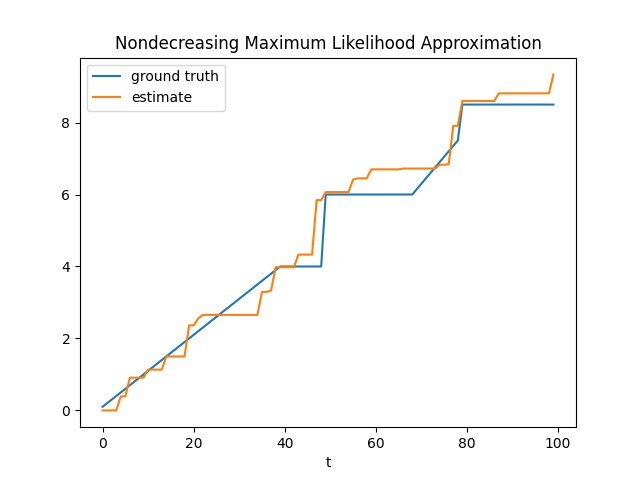
\includegraphics[scale=0.5]{p1_plot_nondecreasing}
    	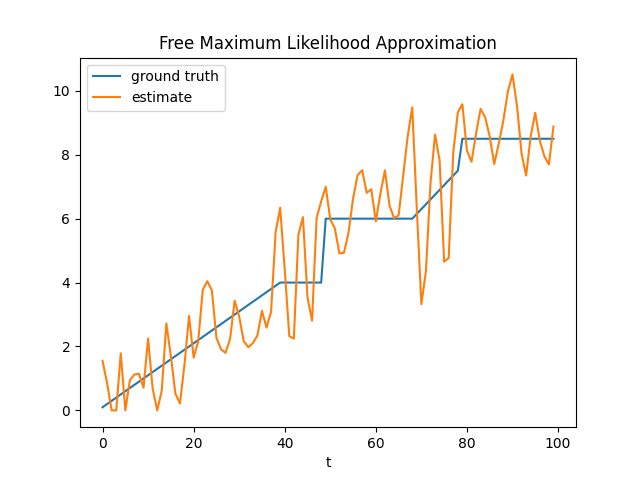
\includegraphics[scale=0.5]{p1_plot_free}
    \end{center}

\item For the maximum likelihood estimate, we want to maximize the log probability function. We know $p_z(u) = \text{exp}(-\phi(\|u\|_2))$, where $\phi : \R \to \R$ is convex and increasing. The density of $x = Az + b$ is given by the hint to be \[
        p_x(v) = \frac{1}{|\text{det}(A)} p_z(A^{-1}(v - b)).
    \] Therefore, the chance of $x_1, \dots, x_N$ is \[
        \prod \frac{1}{|\text{det}(A)} p_z(A^{-1}(x_i - b)).
    \] The log of this probability becomes a sum: \[
        l(\mathbf{x}) = -N \log(|\text{det}(A)|) - \sum_{i=1}^N \phi(\|A^{-1}x_i - A^{-1} b\|_2).
    \] We switch the problem to minimization and multiply $l$ by $-1$. We introduce new variables $u_i$ to clarify. The problem becomes \begin{align*}
        &\text{minimize } N\log(|\text{det}(A)|) + \sum_{i=1}^N u_i \\
        &\text{subject to } \phi(\|A^{-1} b - A^{-1} x_i \|_2) \leq u_i.
    \end{align*} The issue is that the log determinant function is concave. The solution is to make $A^{-1}$ itself be the problem variable rather than $A$. Then the problem becomes instead \begin{align*}
        &\text{minimize } -N\log(\text{det}(Q)) + \sum_{i=1}^N u_i \\
        &\text{subject to } \phi(\|Q b - Q x_i \|_2) \leq u_i,
    \end{align*} where at the end of optimizing for $Q$ we find $A = Q^{-1}$. The problem is DCP if we further assume that $Q$ is positive semidefinite, so that the product $Qb$ is quadratic. Then convex minus affine in the L2 norm is convex. The L2 norm itself is convex, which when passed into $\phi$ remains convex. Therefore the constraints are convex, as is the objective now that we flip the sign of the log determinant.

\end{enumerate}
\end{document}
